The previous sections describe about the importance of Read Copy Update (RCU) in parallel programming paradigm and the rules one should follow to correctly use the RCU primitives. It also describes the violation of RCU rules, which can be a potential bug in program. It also mentions the challenges involved in identifying such bugs and why the existing approaches like static analysis, lock-set based approach etc is not sufficient to identify them.

Our approach to identify the incorrect usage of RCU primitive and possible rcu bugs involves the mechanism of Dynamic Binary Instrumentation (DBI). Dynamic Binary Instrumentation (DBI) is an execution control and analysis technique that involves injecting binary code into a running program. The injected code is term “Instrumentation”. There are many DBI infrastructure exist like DynamoRIO, DynamoRIO Kernel (DRK),  Pin, JIFL, KernInst etc which provides support for fine-grained monitoring and program execution. Our system uses Granary, a comprehensive kernel module instrumentation framework. The choice of Granary as DBI framework is based on the fact that it provides the support for instrumenting only kernel modules and thus incur no overhead when non-module code executes. Granary allows the interaction between the kernel and module through module and kernel wrapper having rich information about kernel and its types, thus giving us the complete control on all the data passed over the wrapper. It also provide the infrastructure for adding watchpoint for all the memory addresses passed over the wrapper. We also decided to evaluate the system by introducing some known bugs while rcu torture test which is build as kernel module and Granary best fit as the DBI framework. 


\subsection{Granary}
Granary is a Dynamic Binary Instrumentation (DBI) framework, developed over DynamoRIO Kernel (DRK) and provides support for fine-grained instrumentation of only kernel modules. Granary gets loaded as the kernel module and interposes during module loading mechanism to generate the module wrapper. It also use the rich kernel type informations to generate a static kernel wrapper. Once the module gets loaded, it runs under the control of Granary and all interactions between the kernel and module happens through one of these wrappers. The presence of these wrappers provides an efficient infrastructure to monitor all the pointers passed from the kernel to the module and add watchpoint on them. The rich kernel type information at the wrapper layer provides support for adding type-based watchpoint on the pointers. However for this project we are using simple watchpoint implementation for tracking the use of RCU primitive and access of RCU protected data. The detail of watchpoint implementation and its usage is provided in next section. 


\subsection{Watchpoint}
Program debugging is a tedious but inevitable chore in software development process. An efficient debugger can make programmers more productive by allowing them to monitor the execution, inspect the state of the process and monitor memory read and write to inspect the data flow and corruption. This increases the requirement of an efficient debugging tool supporting an useful feature called \emph{Watchpoints}. The need of such debugging tool increases, as the complexity of the program grows such as parallel system. \emph{Watchpoint} allow a developer to demarcate a memory region and take control whenever that gets accessed. It then ensures the safe access of the memory addresses by checking certain policy. It is similar to the instruction breakpoints which allows the developer to pause execution at specific instructions.

Implementing software watchpoint, without any architectural support, is expensive since it requires to inspect all memory operations and trigger a callback on the watched addresses. Our system leverages the advances in binary instrumentation and code manipulation technique to provide the efficient feature to add watchpoint at memory addresses. Our system uses this feature to check the correct usage of RCU synchronization primitive and access of RCU protected data, thus identifying the violation of rules and possible buggy usage of RCU.

The naive approach of implementing watchpoint using dynamic binary instrumentation adds new instructions across every memory references to performs the following task: 
\begin{itemize}
	\item Determine the list of addresses which needs to be watched and check if the program is referring to one of the watched addresses.  
	\item Raise a callback when memory operation happens at one of the watched addresses.
	\item Incase the address is not one of the watched addresses, continue the normal execution.
\end{itemize}  
The naive system also maintains a watchlist lookup table to maintain the list of addresses to be watched. It uses an efficient algorithm to look for the addresses in the list before making a callback on watched addresses. One of the drawback of this approach is the runtime overhead, which incurs due to address lookup for every memory addresses. This makes the implementation of watchpoint costly. 

Our system refines the cost of adding watchpoint by substantially reducing the cost of lookup and providing options for faster lookup of meta information in shadow memory. The detail about shadow memory and meta information is provided in next section. We took the advantage of 48 bit implementation in 64-bit architecture and used non-canonical addresses to implement our watchpoint mechanism. The use of non-canonical address provides us the following advantages :
\begin{itemize}
	\item It decreases the cost of lookup as the non-canonical addresses can be easily recognised by masking lower 48 bits of the addresses.
	\item It also provides one to one mapping between the actual address and watched address thus proving virtually no cost for fixing the address.
	\item The unused 15 bits in non-canonical address is used to encode information about the shadow memory storing meta-informations.
	\item The addresses aliasing the watched address also gets watched, thus there is no need to implement a pointer tracking mechanism.
\end{itemize}   

Figure~\ref{fig:addrspace} shows the address-space layout in 64 bit architecture with 48 bit implementations. 
\begin{figure}[h!]
\centering
 	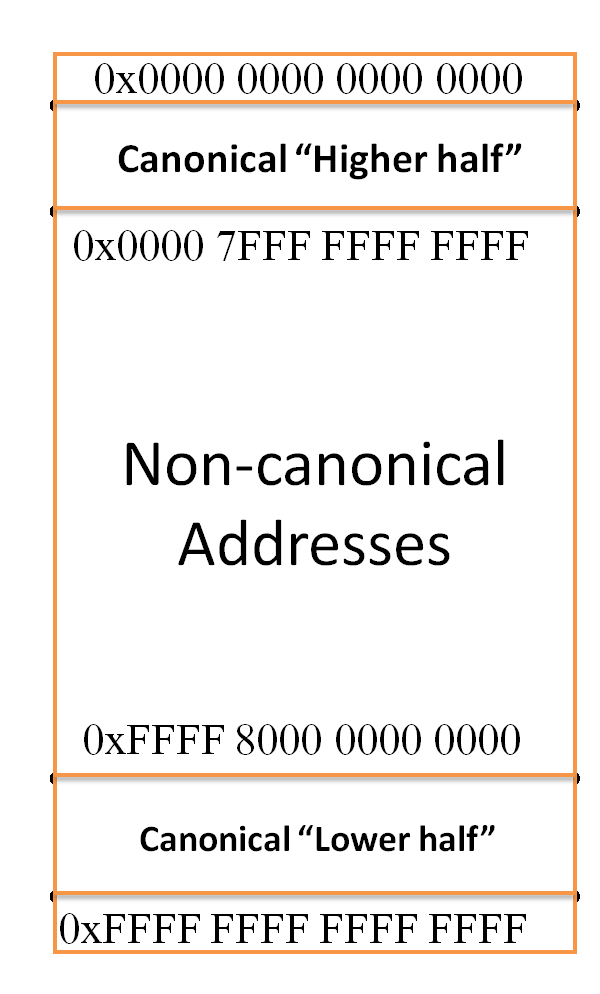
\includegraphics[width=0.2\textwidth]{Picture3-png}
\caption{64-bit address layout (48bit implementation)}\label{fig:addrspace}
\end{figure}
The highest 1 bit (sign bit) is used for adding watchpoint and differentiate between original and watched addresses. The next 15 bit of address is used to for storing shadow memory index storing meta-information. Our method of storing shadow memory index puts a limit on our system in terms of number of active watchpoint we can add at a time, but we consider this is enough for our project to track the rcu protected data. Figure~\ref{fig:watchpoint} shows the detail, how the watched address gets created.

\begin{figure}[h!]
\centering
 	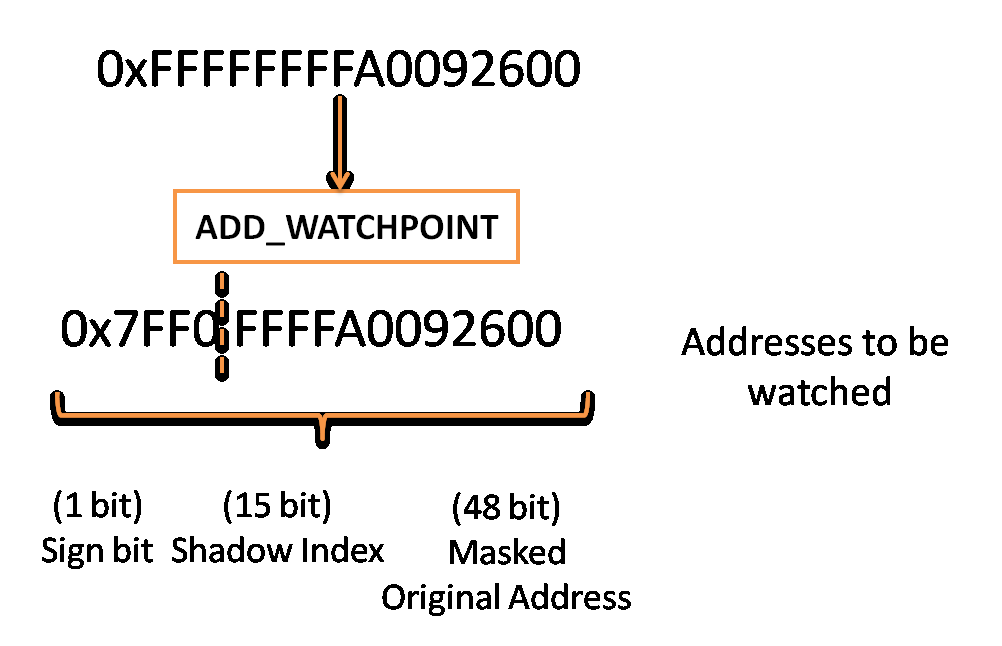
\includegraphics[width=0.4\textwidth]{Picture6-png}
\caption{Watchpoint}\label{fig:watchpoint}
\end{figure}


\subsection {Instrumentation and Optimizations}
Watchpoints essentially requires monitoring of every memory read (load) and write (store) operations. A basic monitoring approach using using dynamic binary instrumentation adds new instructions before every memory references looking for one of the watched address. In our system one of these watched addresses includes the non-canonical addresses generated out of original address and the index of shadow memory storing required meta-information. The detail of watchpoint implementation is provided in previous section. The instrumentation required for implementing watchpoint perform the following operation before every memory references: 

\begin{itemize}
	\item Save and restore the registers that are used or side-effected during watchpoint( stack is used to spill these registers ).
	\item Calculate and check the reference address and check if this is one of the non-canonical addresses.
	\item Inject a callback function taking the original address and shadow memory index as argument, if this is one of the non-canonical one. 
	\item Emulate the actual instruction with corrected address and continue the execution after restoring registers.
	\item Follow the normal course of execution if the address is not one of the watched.
\end{itemize}

\begin{figure}[th!]
%
\framebox{\begin{minipage}[t]{1.02\columnwidth}%
\vspace{-1em}
\begin{codebox}
\Procname{$\proc{Native-Memory-Operation}$}
\li  mov $\id{\%rsi   -> [\%rax, \%rbx]}$ 
\end{codebox}%

\begin{codebox}
\Procname{$\proc{Instrumented-Memory-Operation}$}
\li  	push 	$\id{\%rcx}$
\li  	push 	$\id{\%rdi}$
\li 	lea 	$\id{[\%rax, \%rbx] 	-> 	\%rdi}$
\li 	pushf
\li 	movabs 	$\id{0xffff000000000000		->	\%rcx}$
\li	or 	$\id{\%rcx 	->	\%rdi}$
\li	cmp 	$\id{\%rdi 	->	\%rdi}$
\li	je     	$\id{addr\_not\_watchpoint}$
\li	popf
\li 	$\proc{insert\_clean\_call}(\id{watch\_write}, \id{\%rdi}, \id{1})$
\li	mov    	$\id{\%rsi	->	[\%rdi]}$
\li	pop	$\id{\%rdi}$
\li	pop 	$\id{\%rcx}$
\li	jmp 	$\id{done\_instrumenting}$
\li	LABEL:  $\id{addr\_not\_watchpoint}$
\li	popf
\li	pop	$\id{\%rdi}$
\li	pop 	$\id{\%rcx}$
\li  	mov 	$\id{\%rsi   	-> 	[\%rax, \%rbx]}$ 
\li	LABEL:  $\id{done\_instrumenting}$
\li  	nop	
\end{codebox}%
\end{minipage}}

\caption{Native and Instrumented memory write Operation\label{fig:mem-write}}
\vspace{-1em}
\end{figure}

Figure~\ref{fig:mem-write} shows the example of native and a naive version of instrumented code for memory write operation. The naive instrumented code described above suffers from a significant runtime overhead. We implemented and applied some of the optimization to systematically improve the runtime performance. We used the following optimizations: 
\begin{itemize}
	\item \emph{Dead Registers Analysis : }Every instrumentation system needs scratch registers for creating and injecting new instructions. These registers can be obtained by spilling them to memory locations. Our naive instrumentation uses stack to spill these registers. The frequent spilling of these registers on stack or memory location increases the cost of instrumentation significantly. Our system performs the register liveness analysis on each basic block to identify registers that can be safely used without requiring it to spill on the stack. For register liveness analysis, our system starts instrumenting from the end of the basicblock moving upward and collecting all the source and destination registers making all the non source and non base-displacement registers (whole destination registers) as dead.  
	\item \emph{Flag Liveness Analysis : } In the above example for naive instrumentation, we also need to save and restore the flags as the instrumented code modifies the flag. One important optimization in instrumentation is Flag Liveness analysis and we save and restore the flag only when it is alive. To identify the dead flag as we move from upward instrumenting basic block, we find if any of the instruction modify the flags we consider the instruction previous to that as having dead flag. 
	\item \emph{Merge Checks :} We also exploited the locality of memory references and two instructions in the same basic block accessing the same object or different member of same object (like \emph{0x0(\%rax) and 0x8(\%rax)}) doesn’t require the instrumentation of all references and thus the checks for all of them is merged together.
    \item \emph{Eliminate Stack Operations :} For x86 architecture, any operation on the stack or involving stack pointer is considered as the memory operation. Our system identify all these instructions involving operations on the stack and they are not required to be instrumented since we are not tracking or adding watchpoint on them.
\end{itemize}

The optimization discussed above improved the performance of watchpoint significantly, but there is a scope of further optimization and one of them is policy based instrumentation. Policy based instrumentation will only instruments the memory references when execution enters in RCU critical section and any access outside critical section is incorrect and will get trapped by the general protection fault. However this is a big optimization but we have not implemented this since it requires implementation of basic block tagging mechanism to have two version of basicblock for same native code , which is currently not supported with Granary.


\subsection{Shadow memory and meta information}
Implementing shadow memory and use of meta-information is important for tracking RCU primitive and verifying memory access policy for RCU protected data. This section describes detail about the type of meta-information we used and how it is important for tracking the usage of RCU synchronization primitive. The two types of meta-information used are follows: 
\begin{itemize}
 	\item \emph{Per thread meta-information :} It includes thread generation number which gets stored at thread local slot created at the bottom of the stack. The thread generation number keeps track of the rcu read critical section and used to validate the correct usage of RCU protected data.
   	\item \emph{Per pointer meta-information :} It includes watchpoint generation number and writer\_thread\_id.  Watchpoint generation number along with thread generation number is used to decide the memory access policy. It also stores the information if the watchpoint pointer is source or one of the alias of source pointer generated by \emph{rcu\_dereference()}. The structure of the per pointer meta-information is shown in the figure~\ref{fig:metainfo}. 
\end{itemize} 

The per pointer meta-information gets stored in the shadow memory. As shown in figure~\ref{fig:metainfo} the shadow memory stores a large array of \emph{union alias\_meta} which includes \emph{ alias\_meta\_thread *thread\_info} as one of its element. The \emph{thread\_info} stores the writer thread id who allocates and allowed to update the memory location before `publish` happens. It also stores the watchpoint generation number for each thread. 

Shadow memory provides an efficient infrastructure for implementing watchpoint mechanism. In our approach of implementing shadow memory we split and reserve a part of address space as shadow memory. Shadow memory stores a large array of meta information type \emph{union alias\_meta}, the index of which is used for creating watchpoint address. Our approach of using shadow memory is efficient as we can directly access the corresponding watchpoint meta-information using shadow index. 

\begin{figure*}[h]
%\centering
\begin{lstlisting}
/* Thread-specific watchpoint meta information. */
struct alias_meta_thread {
    // for linking in the free list.
    alias_meta_thread *next;

    /* writer thread_id + 1 iff this RCU-protected structure is being
     * written to; otherwise 0. An RCU-protected structure is writable from
     * the time of allocation up until it is published using rcu_assign_pointer.
     */
    uint64_t writer_thread_id;

    /* The "generation" number of the thread */
    uint64_t gen_nums[NUM_THREADS];
};

union alias_meta {
        // if this watchpoint aliases another watchpoint
        alias_meta *source;
        /* thread info about a source watchpoint */
        alias_meta_thread *thread_info;
}; 
\end{lstlisting}
\caption{Meta-Information: data structure used for meta-info}\label{fig:metainfo}
\end{figure*}

The shadow memory stores a large array of meta information which can be accessed by the index stored with the watchpoint. The meta-information gets generated and stored during the rcu data allocation and its index is used to generate watched address. Our meta-information also keeps track of pointer aliasing. The two elements \emph{source} and emph{thread\_info} helps in tracking the pointer aliasing which is particularly useful in tracking rcu bugs violating rule 1 \emph{TODO : check this}. 

The meta-information contains the thread specific generation number and writer \emph{thread\_id} which is allowed to modify it before publish. These thread specific meta-information gets generated at runtime while adding watchpoint. The figure below shows the structure of per-pointer meta-information. 

Apart from the per-pointer meta-information we also store the per-thread meta information. These per-thread information gets stored at the thread local slots created at the bottom of the stack. These thread-local-storage (TLS) is also used to store the generation number which is then used to check the correct usage of RCU.

\subsection{Page fault handler}
To implement our watchpoint we used non-canonical addresses which gets generated out of actual memory address and the shadow memory index. Our system uses binary instrumentation to find out any such addresses and fixes it to get the correct address before memory operation. We are using Granary, a comprehensive kernel module instrumentation framework, which only rewrites the kernel module code and loses its control when non-module code executes. This makes it possible to leak any of these addresses to leak to the kernel which when accessed causes general protection fault. To handle such cases our system takes control of interrupt handler and gives a callback in case of general protection fault. This callbacks checks for any such watched addresses in registers and the stack and fixes them before doing \emph{iret}. The callback also prevents call to kernel general-protection fault in such cases which prevents any overhead due to kernel general protection fault handler. We tested the changes we did in page-fault handler with different modules but in-case of rcutorture module we have not encountered any such addresses leaking to the kernel.

